% Standalone proposed cross-attention architecture. Compile with pdfLaTeX.
\documentclass[11pt]{article}
\usepackage[paperwidth=26cm,paperheight=17cm,margin=5mm]{geometry}
\usepackage[T1]{fontenc}
\usepackage{lmodern,amsmath,amssymb,tikz}
\usetikzlibrary{arrows.meta,calc}
\pagestyle{empty}
\definecolor{outline}{HTML}{153543}
\definecolor{norm}{HTML}{B9CDD0}
\definecolor{attn}{HTML}{ECE6D8}
\definecolor{ffn}{HTML}{B9B2C4}
\definecolor{linear}{HTML}{D8B5BE}
\definecolor{reference}{HTML}{C9BEDA}
\begin{document}
\noindent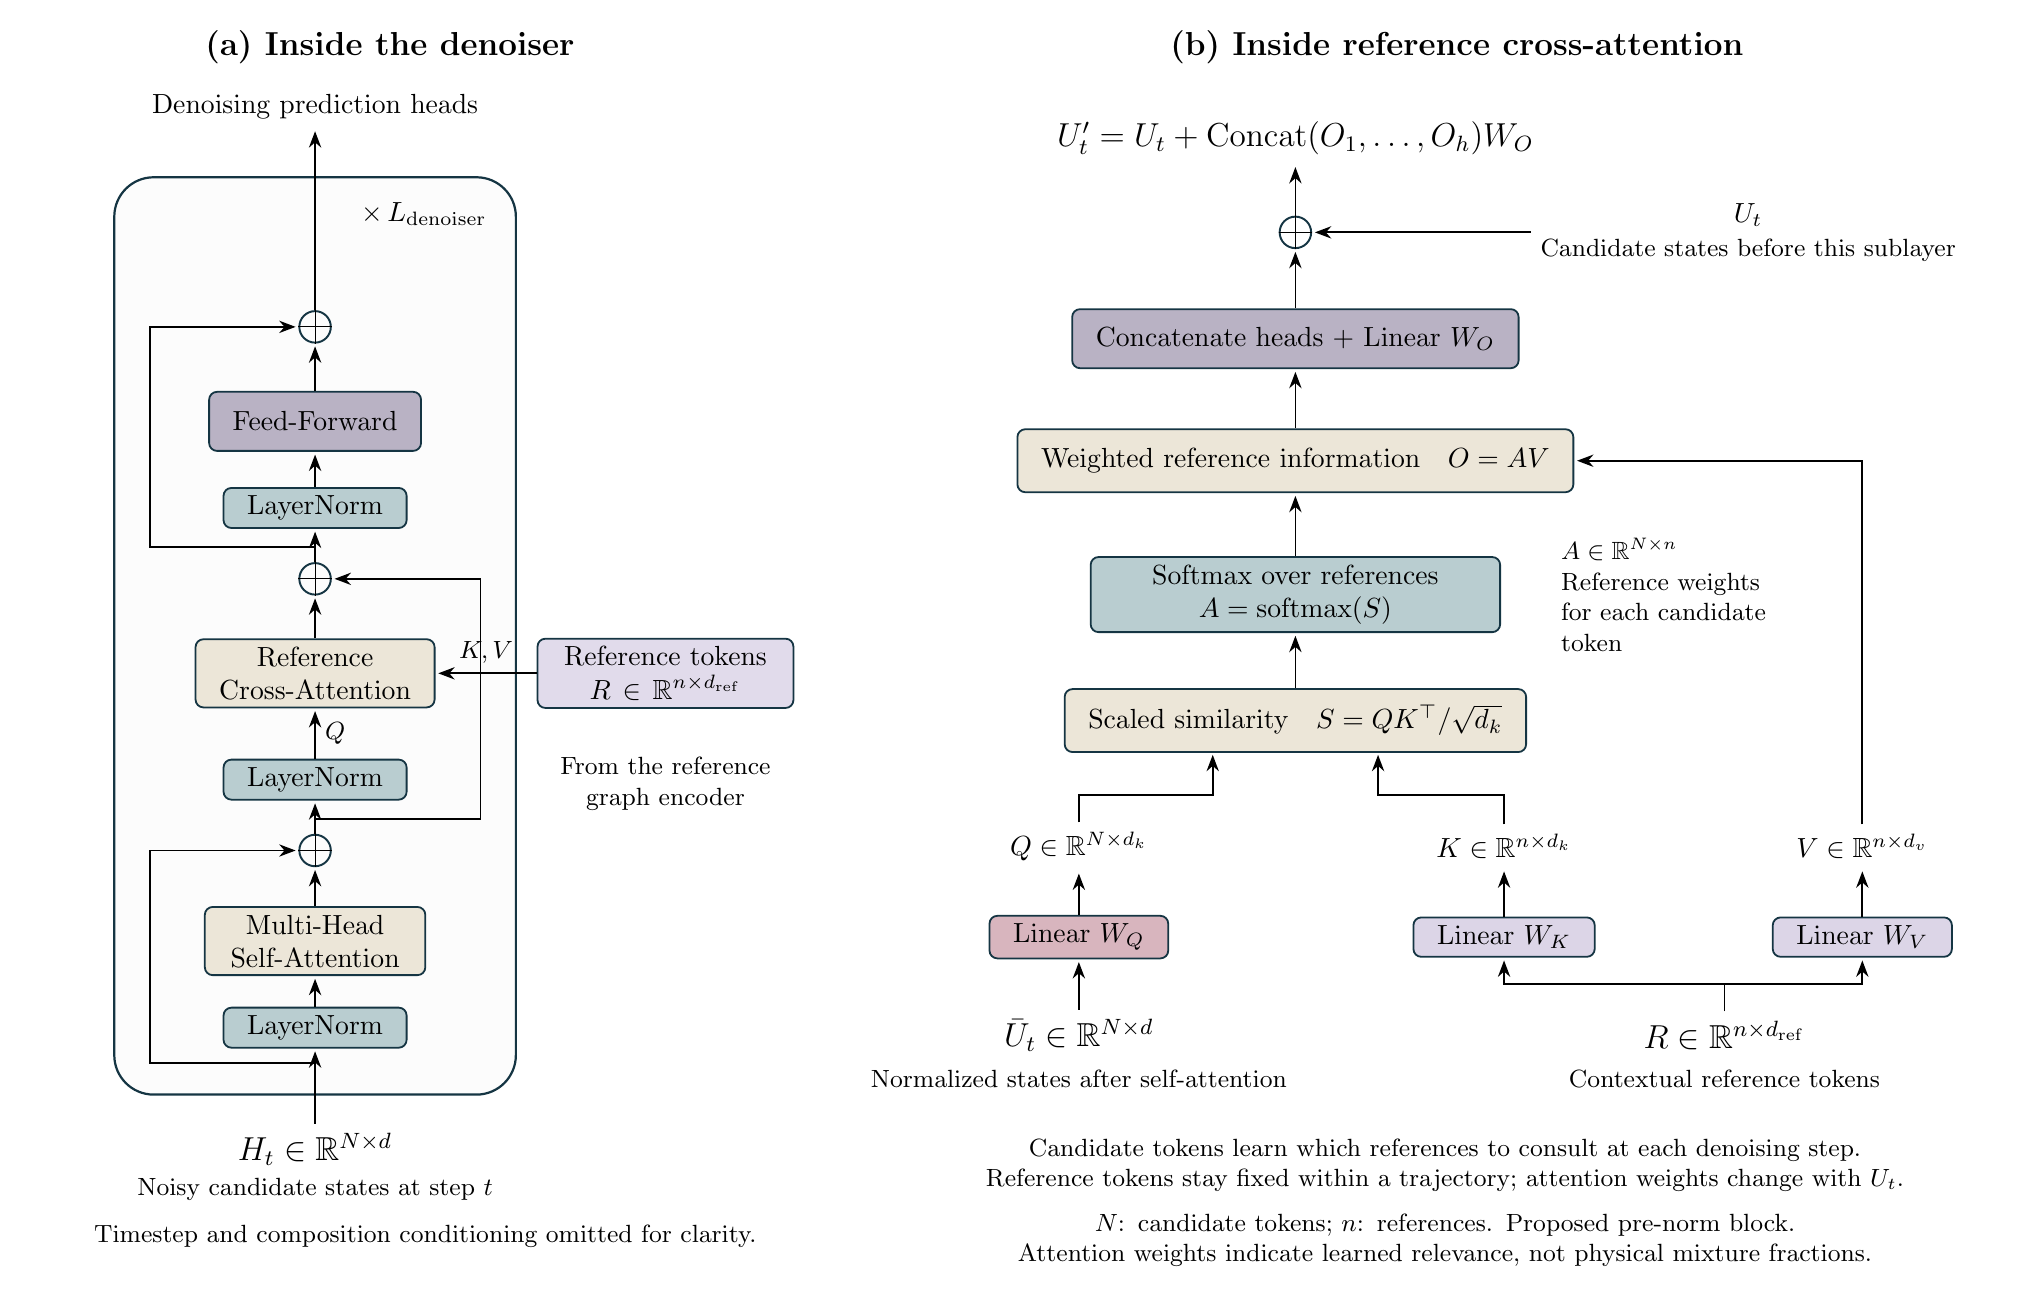
\begin{tikzpicture}[x=1cm,y=1cm,>=Stealth,
 layer/.style={draw=outline,line width=.65pt,rounded corners=1mm,align=center,minimum height=.5cm,inner xsep=3mm,inner ysep=1mm},
 arrow/.style={->,line width=.65pt,shorten >=1pt},
 add/.style={circle,draw=outline,line width=.7pt,minimum size=4mm,inner sep=0pt}]
\path[use as bounding box] (0,0) rectangle (25,15.8);

% Panel a: reference-conditioned block inside the denoising transformer.
\node[font=\large] (hin) at (3.65,1.55) {$H_t\in\mathbb R^{N\times d}$};
\node[font=\small] at (3.65,1.05) {Noisy candidate states at step $t$};
\draw[draw=outline,rounded corners=5mm,line width=.8pt,fill=black!1]
 (1.1,2.25) rectangle (6.2,13.9);
\node[anchor=north east] at (5.95,13.7) {$\times\,L_{\mathrm{denoiser}}$};
\node[layer,fill=norm] (ln1) at (3.65,3.1) {LayerNorm};
\node[layer,fill=attn,minimum width=2.8cm,minimum height=.85cm] (sa) at (3.65,4.2) {Multi-Head\\Self-Attention};
\node[add] (sum1) at (3.65,5.35) {};
\node[layer,fill=norm] (ln2) at (3.65,6.25) {LayerNorm};
\node[layer,fill=attn,minimum width=2.8cm,minimum height=.85cm] (ca) at (3.65,7.6) {Reference\\Cross-Attention};
\node[add] (sum2) at (3.65,8.8) {};
\node[layer,fill=norm] (ln3) at (3.65,9.7) {LayerNorm};
\node[layer,fill=ffn,minimum width=2.65cm,minimum height=.75cm] (ff) at (3.65,10.8) {Feed-Forward};
\node[add] (sum3) at (3.65,12.0) {};
\foreach \s in {sum1,sum2,sum3}{\draw (\s.west)--(\s.east) (\s.south)--(\s.north);}
\draw[arrow] (hin)--(ln1);
\draw[arrow] (ln1)--(sa);
\draw[arrow] (sa)--(sum1);
\draw[arrow] (sum1)--(ln2);
\draw[arrow] (ln2)--node[right,font=\small] {$Q$} (ca);
\draw[arrow] (ca)--(sum2);
\draw[arrow] (sum2)--(ln3);
\draw[arrow] (ln3)--(ff);
\draw[arrow] (ff)--(sum3);
\draw[arrow] (3.65,2.65)--(1.55,2.65)|-(sum1.west);
\draw[arrow] (3.65,5.75)--(5.75,5.75)|-(sum2.east);
\draw[arrow] (3.65,9.2)--(1.55,9.2)|-(sum3.west);
\node[align=center] (head) at (3.65,14.8) {Denoising prediction heads};
\draw[arrow] (sum3)--(head);
\node[layer,fill=reference!55,align=center,text width=2.65cm] (ref) at (8.1,7.6)
 {Reference tokens\\$R\in\mathbb R^{n\times d_{\mathrm{ref}}}$};
\draw[arrow] (ref.west)--node[above,font=\small] {$K,V$} (ca.east);
\node[align=center,font=\small,text width=3.1cm] at (8.1,6.2) {From the reference\\graph encoder};
\node[align=center,font=\small,text width=8.5cm] at (5.05,.45)
 {Timestep and composition conditioning omitted for clarity.};
\node[font=\large\bfseries] at (4.6,15.55) {(a) Inside the denoiser};

% Panel b: expanded cross-attention. All dimensions are per head unless stated.
\node[font=\large\bfseries] at (18.15,15.55) {(b) Inside reference cross-attention};
\node[font=\large] (candidate) at (13.35,3.0) {$\bar U_t\in\mathbb R^{N\times d}$};
\node[font=\small] at (13.35,2.45) {Normalized states after self-attention};
\node[font=\large] (rtokens) at (21.55,3.0) {$R\in\mathbb R^{n\times d_{\mathrm{ref}}}$};
\node[font=\small] at (21.55,2.45) {Contextual reference tokens};
\node[layer,fill=linear] (wq) at (13.35,4.25) {Linear $W_Q$};
\node[layer,fill=reference!65] (wk) at (18.75,4.25) {Linear $W_K$};
\node[layer,fill=reference!65] (wv) at (23.3,4.25) {Linear $W_V$};
\draw[arrow] (candidate)--(wq);
\draw[arrow] (rtokens.north)--(21.55,3.65)-|(wk.south);
\draw[arrow] (21.55,3.65)-|(wv.south);
\node (q) at (13.35,5.4) {$Q\in\mathbb R^{N\times d_k}$};
\node (k) at (18.75,5.4) {$K\in\mathbb R^{n\times d_k}$};
\node (v) at (23.3,5.4) {$V\in\mathbb R^{n\times d_v}$};
\draw[arrow] (wq)--(q);
\draw[arrow] (wk)--(k);
\draw[arrow] (wv)--(v);
\node[layer,fill=attn,minimum width=5.2cm,minimum height=.8cm] (score) at (16.1,7.0)
 {Scaled similarity\quad $S=QK^\top/\sqrt{d_k}$};
\draw[arrow] (q.north)--(13.35,6.05)-|(15.05,6.6);
\draw[arrow] (k.north)--(18.75,6.05)-|(17.15,6.6);
\node[layer,fill=norm,minimum width=5.2cm,minimum height=.75cm] (softmax) at (16.1,8.6)
 {Softmax over references\\$A=\mathrm{softmax}(S)$};
\draw[arrow] (score)--(softmax);
\node[anchor=west,align=left,font=\small,text width=3cm] at (19.35,8.6)
 {$A\in\mathbb R^{N\times n}$\\Reference weights for each candidate token};
\node[layer,fill=attn,minimum width=5.2cm,minimum height=.8cm] (weighted) at (16.1,10.3)
 {Weighted reference information\quad $O=AV$};
\draw[arrow] (softmax)--(weighted);
\draw[arrow] (v.north)--(23.3,10.3)--(weighted.east);
\node[layer,fill=ffn,minimum width=5.2cm,minimum height=.75cm] (heads) at (16.1,11.85)
 {Concatenate heads + Linear $W_O$};
\draw[arrow] (weighted)--(heads);
\node[add] (res) at (16.1,13.2) {};
\draw (res.west)--(res.east) (res.south)--(res.north);
\draw[arrow] (heads)--(res);
\node[align=center] (skip) at (21.85,13.2) {$U_t$\\\small Candidate states before this sublayer};
\draw[arrow] (skip.west)--(res.east);
\node[font=\large] (hout) at (16.1,14.4) {$U'_t=U_t+\mathrm{Concat}(O_1,\ldots,O_h)W_O$};
\draw[arrow] (res)--(hout);
\node[align=center,font=\small,text width=12.7cm] at (18.0,1.35)
 {Candidate tokens learn which references to consult at each denoising step.\\Reference tokens stay fixed within a trajectory; attention weights change with $U_t$.};
\node[align=center,font=\small,text width=12.7cm] at (18.0,.4)
 {$N$: candidate tokens; $n$: references. Proposed pre-norm block.\\Attention weights indicate learned relevance, not physical mixture fractions.};
\end{tikzpicture}
\end{document}
